\documentclass[letterpaper, 10 pt, conference]{ieeeconf}  
\IEEEoverridecommandlockouts
\usepackage{enumerate}
\usepackage{graphicx}

\title{Dynamic Manipulation in Task-Level Planning}
\author{}

\begin{document}
\maketitle

\section{Introduction}

\begin{figure*}[ht!] 
  \centering
  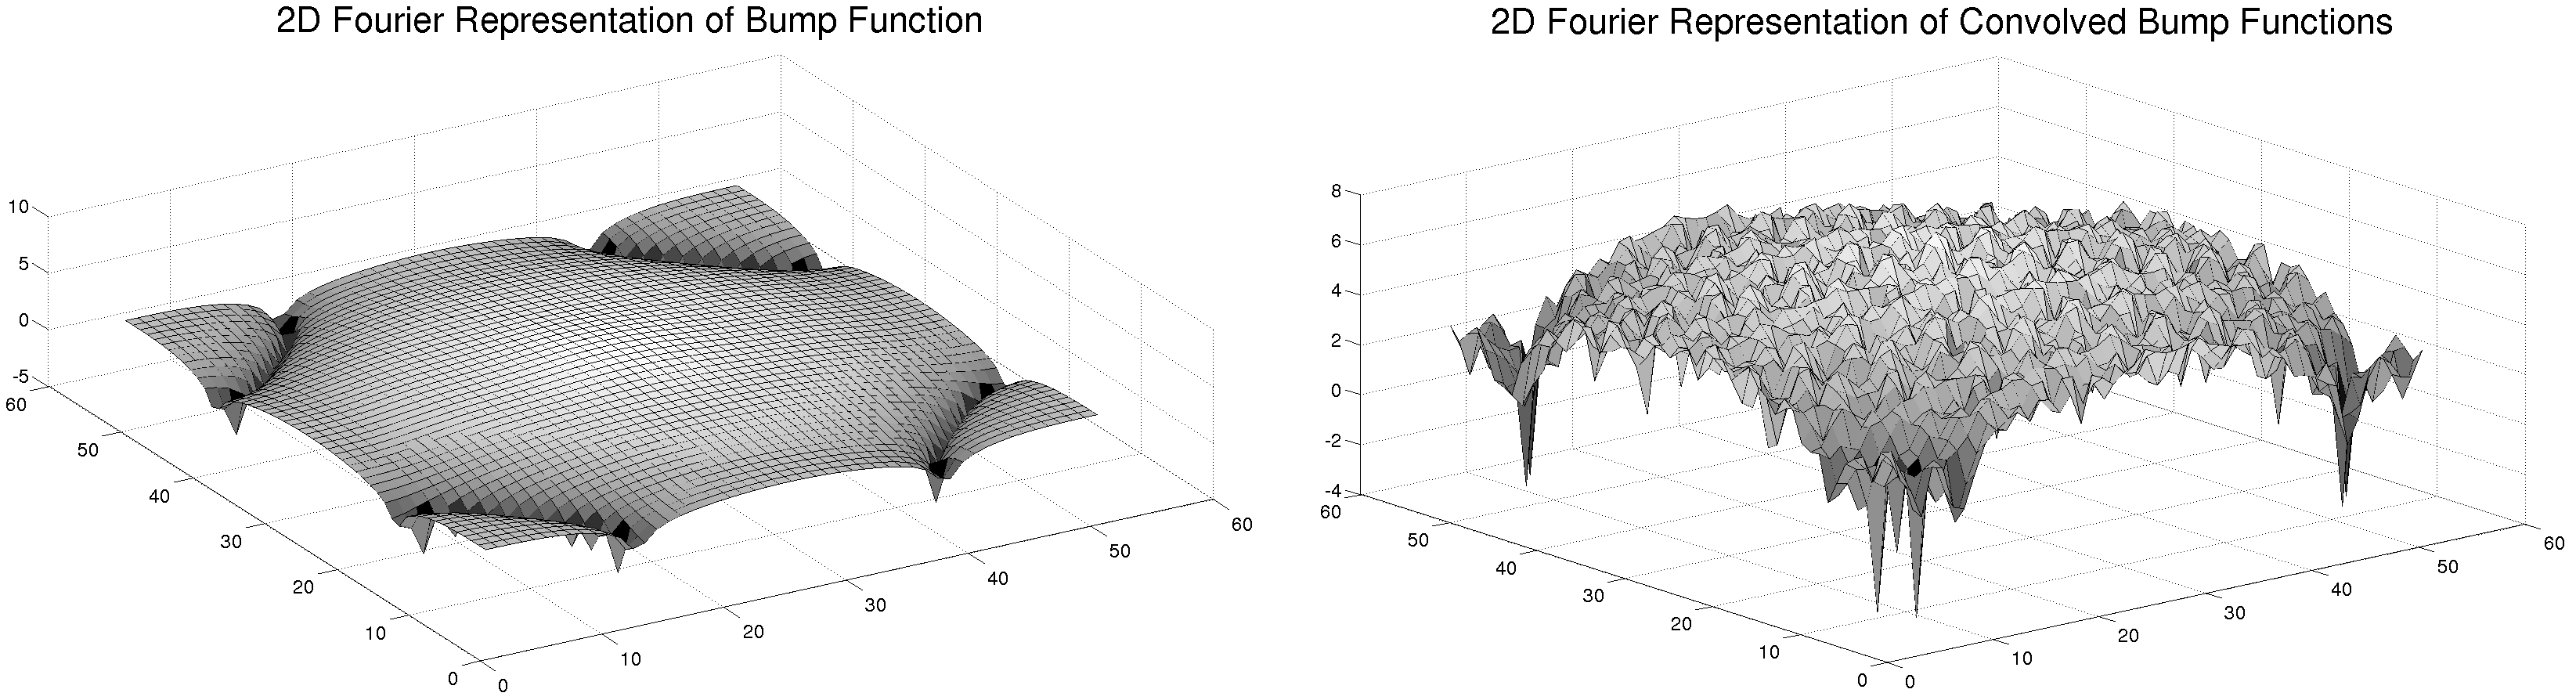
\includegraphics[width=1.0\linewidth]{Figures/bumpFouriers.png}
  \caption{An example of a gear chain designed to transmit mechanical power from the 
  input gear (green) to the output gear (blue) using spur (yellow, cyan) and worm gears (black) and avoiding
  obstacles (red).}
  \label{fig:main}
\end{figure*}

% \bibliographystyle{unsrt}
% \bibliography{dynamic-references}

\end{document}

% The nature of the constraints that bind objects together is dependent on the choice of surface-edge matches.
